\section{Context} \subsection{}\label{}

\begin{frame}{General context in visual recognition}
	
	
	\begin{block}{\small Big Data, images are omnipresent}
		\vspace{-0.5cm}
		\begin{table}[t]	
			\centering
			\tiny
			\begin{tabular}{c c c}
				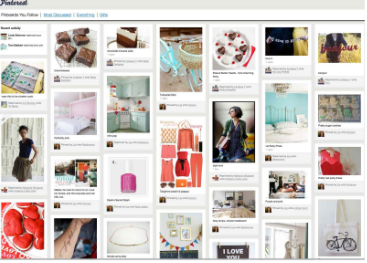
\includegraphics[scale=0.12]{images/bigdatab.png} &
				
\includegraphics[scale=0.12]{images/bigdataa.png} &
				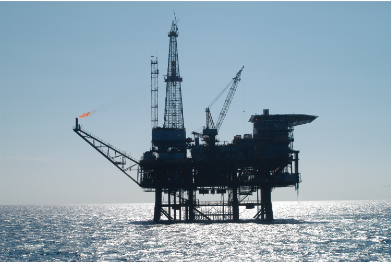
\includegraphics[scale=0.12]{images/bigdatac.png} \\
				Facebook: $\sim$ 1B images/day &
				BBC: > 2.4M videos &
				> 100M monitoring cameras
			\end{tabular}
		\end{table}
		\vspace{-0.3cm}
		\footnotesize
		Methods to process visual datasets:
		\begin{itemize}
			\item Before 2012: hand crafted models, SIFT, SVM
			\item After 2012: \textbf{Convolutional Neural Networks} 
			\item Thanks to research, GPUs, large datasets, and libs (Torch, Theano, etc.)
		\end{itemize}
	\end{block}
	
	\vspace{-0.4cm}

	\begin{figure}[h]
		\centering
		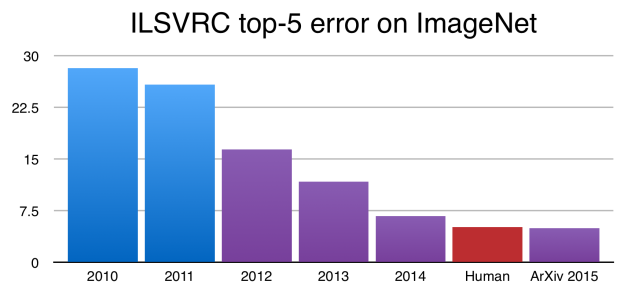
\includegraphics[width=.55\linewidth]{images/ILSVRC.png}
		\label{fig:quora-invariance-1}
	\end{figure}
		

\end{frame}

%--

\begin{frame}{Usual methods on medium and small datasets}
	
	\begin{figure}[h]
		\centering
		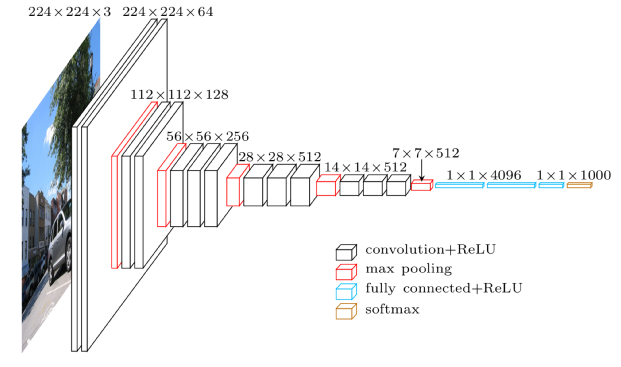
\includegraphics[width=.79\linewidth]{images/vgg16.png}
		\caption{\small Vgg16 \cite{simonyan2014very}, top2 ILSVRC2014}
		\label{fig:quora-invariance-1}
	\end{figure}
	
	\vspace{-0.6cm}
	
	\begin{itemize}
		\item \textbf{From Scratch} : (re)initialization + train with SGD
		\item \textbf{Extraction} : pretrain model + train a linear model (SVM)
		\item \textbf{Fine Tuning} : pretrain model + train with SGD
	\end{itemize}

\end{frame}

\begin{frame}{CNNs benchmark}
	
	\begin{table}[h]
		\centering
		\resizebox{300pt}{!}{%
			\begin{tabular}{|c|c|c|c|c|c|}
				\hline
				Model & Input & Param. & Depth & Implem. & Time (ms) \\ \hline \hline
				Overfeat & 221 & 145M & 9 & GPU & 1,005.63 \\
				Vgg16 & 224 & 138M & 16 & GPU & 1,602.96 \\
				InceptionV3 & 399 & 24M & 42 & GPU & \textbf{978.01} \\ \hline
				InceptionV3 & 399 & 24M & 42 & CPU & 88,262.84 \\
				\hline
			\end{tabular}}
			\caption{\small Forward+Backward with batches of 50 images.} 
			\label{table:cnnbenchmark}
		\end{table}
		
\end{frame}

% --

\section{Medium datasets} \subsection{}\label{}
% --
\begin{frame}{Example : UPMC Food101 (Medium dataset)}
	
	\hspace{0.5cm}\href{http://visiir.lip6.fr}{\textbf{Try our demo on \underline{visiir.lip6.fr} ! \tiny{(designed for Smartphone and Computer)}}}
	
	\vspace{-.2cm}
	
	\begin{figure}
		\centering
		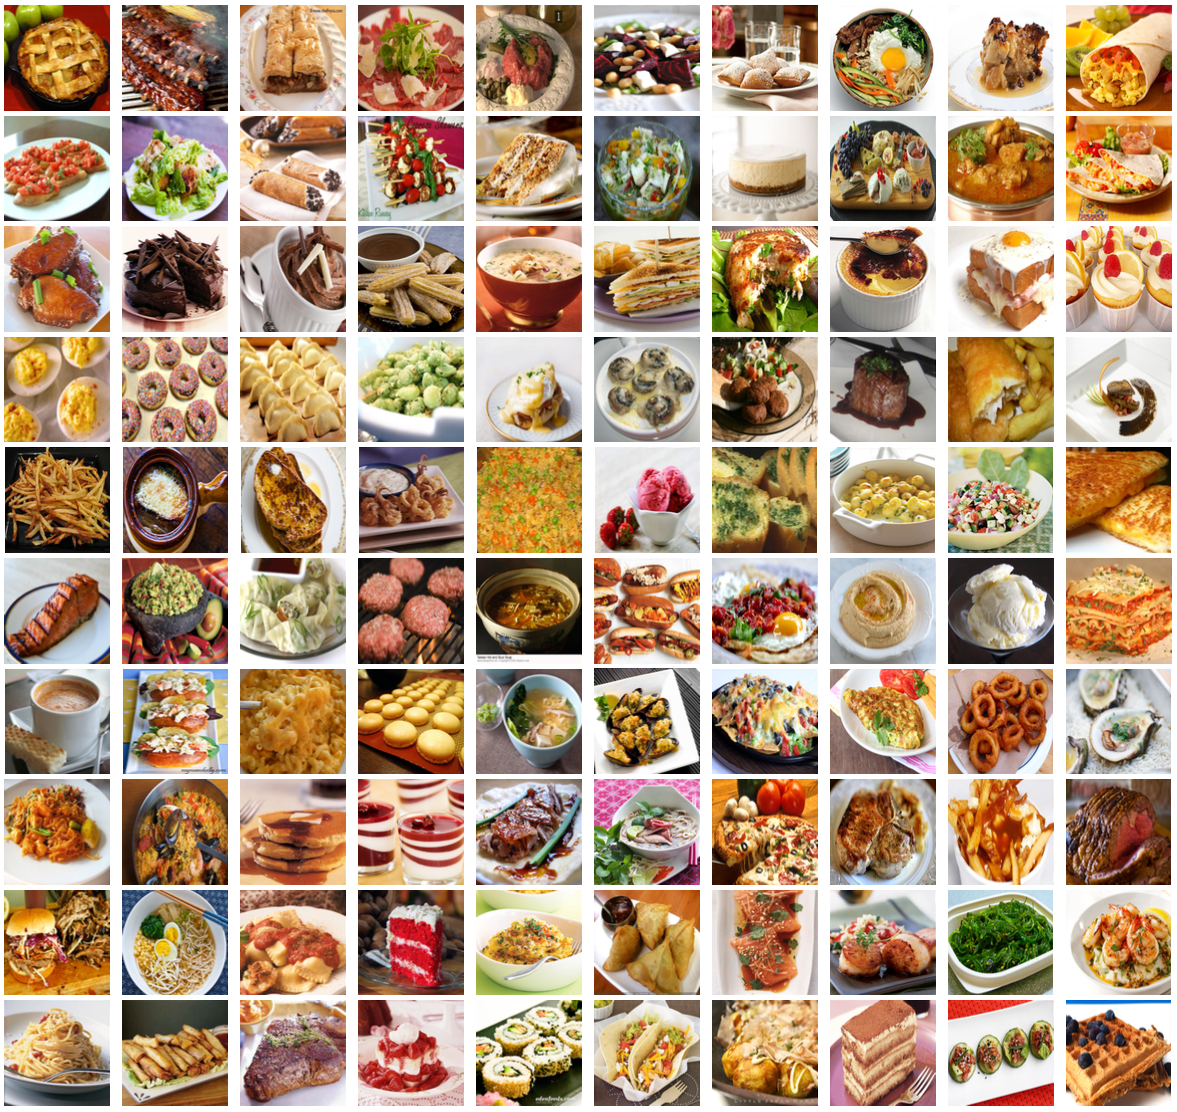
\includegraphics[width=.60\linewidth]{images/UPMC_Food101.png}
%		\caption{80000 train images, 20000 test images, 101 classes}
		\label{fig:2images}
	\end{figure}
	
	\vspace{-0.4cm}
	
	\hspace{1.3cm}80,000 train images, 20,000 test images, 101 classes
	
\end{frame}

\begin{frame}{Results : UPMC Food101 (Medium dataset)}
	
	\begin{table}[h]
		\centering
		\resizebox{220pt}{!}{%
			\begin{tabular}{|c|c|c|}
				\hline
				Model & Method & Test Top1 (\%) \\ \hline \hline
				* BoW \& SVM & Hand Crafted & 28.59 \\ \hline
				* Overfeat \& SVM & Extraction & 33.91 \\
				Overfeat & From Scratch & 47.46 \\
				Overfeat & Fine Tuning & 57.98  \\ \hline
				* Vgg16 \& SVM & Extraction & 40.21  \\
				Vgg16 & From Scratch & 53.62  \\
				Vgg16 & Fine Tuning & 65.71 \\ \hline
				InceptionV3 & Fine Tuning & \textbf{66.83} \\
				\hline
			\end{tabular}}
			%\caption{Pourcentage de bonnes classification.}
			\label{table:upmc1}
		\end{table}
		
		\vspace{-0.3cm}
		
		\hspace{1.6cm} \small{* optimized by \cite{wang2015recipe} }
		
		\begin{itemize}
			\item \textbf{Fine Tuning > All}
			\item From Scratch > Extraction
			\item Very Deep > Deep
		\end{itemize}
\end{frame}

\section{Small datasets} \subsection{}\label{}

\begin{frame}{Example : DSG online (Small dataset)}
	
	Data Science Game (DSG) Online Challenge
	
	\textbf{1st team /117 on the \href{https://inclass.kaggle.com/c/data-science-game-2016-online-selection/leaderboard}{\underline{private leaderboard}}}
	
	\begin{figure}
		\centering
		\begin{subfigure}{.23\textwidth}
			\centering
			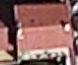
\includegraphics[width=.75\linewidth]{images/dsg1.jpg}
			%			\caption{\small North-South (3479)}
			\label{fig:dsg1}
		\end{subfigure}%
		\begin{subfigure}{.23\textwidth}
			\centering
			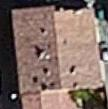
\includegraphics[width=.75\linewidth]{images/dsg2.jpg}
			%		\caption{\small East-West (1856)}
			\label{fig:dsg2}
		\end{subfigure}
		\begin{subfigure}{.23\textwidth}
			\centering
			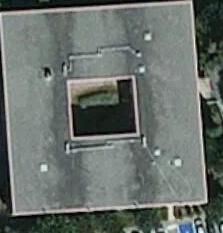
\includegraphics[width=.75\linewidth]{images/dsg3.jpg}
			%		\caption{\small Flat (859)}
			\label{fig:dsg3}
		\end{subfigure}
		\begin{subfigure}{.23\textwidth}
			\centering
			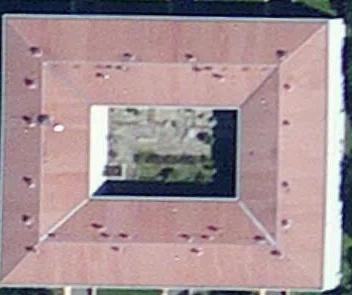
\includegraphics[width=.75\linewidth]{images/dsg4.jpg}
			%		\caption{\small Other (1806)}
			\label{fig:dsg4}
		\end{subfigure}
%		\caption{8000 train images, 20760 no label, 13999 test images}
		\label{fig:dsgimages}
	\end{figure}

	\vspace{-.4cm}

	\hspace{.4cm} north-south \hspace{.6cm} east-west \hspace{1.3cm} flat \hspace{1.6cm} other

	\begin{itemize}
		\item 8,000 train images
		%\item 20,760 train images no label
		\item 13,999 test images
		\item 4 classes
	\end{itemize}
	
\end{frame}

%--

\begin{frame}{Results : DSG Online (Small dataset)}
	
	\href{https://inclass.kaggle.com/c/data-science-game-2016-online-selection/forums/t/22148/sharing-of-knowledge/126808\#post126808}{More details on our winning solution on the \underline{competition forum}}
	
	\vspace{-.5cm}
	
	\begin{table}[H]
		\centering
		\resizebox{320pt}{!}{%
		\begin{tabular}{|c|c|c|}
			\hline
			Model & Method & Test Top1 (\%) \\ \hline \hline
			* BoW \& SVM & Ensemble \& Hand Crafted & 72.40 \\
			* Vgg16 \& SVM & Extraction & 79.00 \\
			Vgg16 &  Fine Tuning & 81.37 \\
			InceptionV3 & Fine Tuning & 82.61\\
			* Custom CNNs & Ensemble \& From Scratch & 84.38 \\
			* Custom CNNs \& Vgg16 & Ensemble \& From Scratch \& Fine Tuning & 85.14 \\
			\textbf{InceptionV3} & \textbf{Ensemble \& Fine Tuning} & \textbf{86.58}\\
			\hline
		\end{tabular}}
		%\caption{}
		\label{table:voc3}
	\end{table}
	
	\vspace{-0.5cm}
	
	\hspace{1cm} \small{* optimized by other competitors}
	
	\begin{itemize}
		\item \textbf{Fine Tuning > All}
		\item Ensembling primordial
		\item From Scratch Custom > Extraction
	\end{itemize}
\end{frame}

%--
\iffalse
\begin{frame}{Evaluation of usual methods: Conclusion}

	\begin{itemize}
		\item Using GPUs is primordial (factor of 80)
		\item Adam works well
		\item \textbf{Fine Tuning > All}
		\item \textbf{Medium dataset: From Scratch > Extraction}
		\item \textbf{Small dataset: Extraction > From Scratch  }
		\item \textbf{Small dataset: Ensembling is primordial}
	\end{itemize}

\end{frame}
\fi



\section{Strong spatial variance} \subsection{}\label{}

%--

\begin{frame}{How CNNs achieve translation invariance}
	
	\begin{figure}[h]
		\centering
		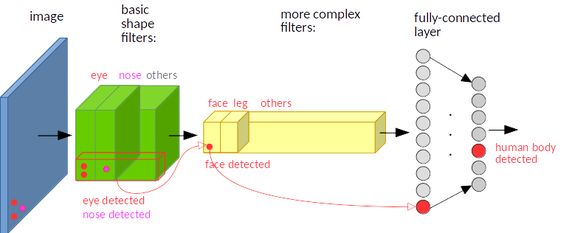
\includegraphics[width=.80\linewidth]{images/quora-invariance-1.png}
		\label{fig:quora-invariance-1}
	\end{figure}
	
	\vspace{-0.5cm}
	
	\begin{figure}[h]
		\centering
		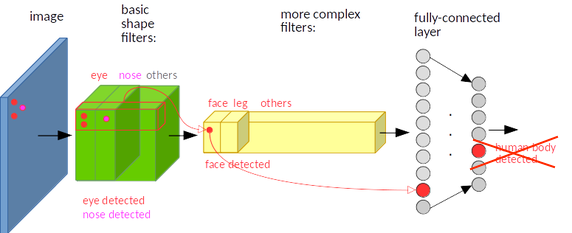
\includegraphics[width=.80\linewidth]{images/quora-invariance-2.png}
		\label{fig:quora-invariance-2}
	\end{figure}
	
\end{frame}

%--

\begin{frame}{Multi Instance Learning: WELDON}
	\begin{figure}[h]
		\centering
		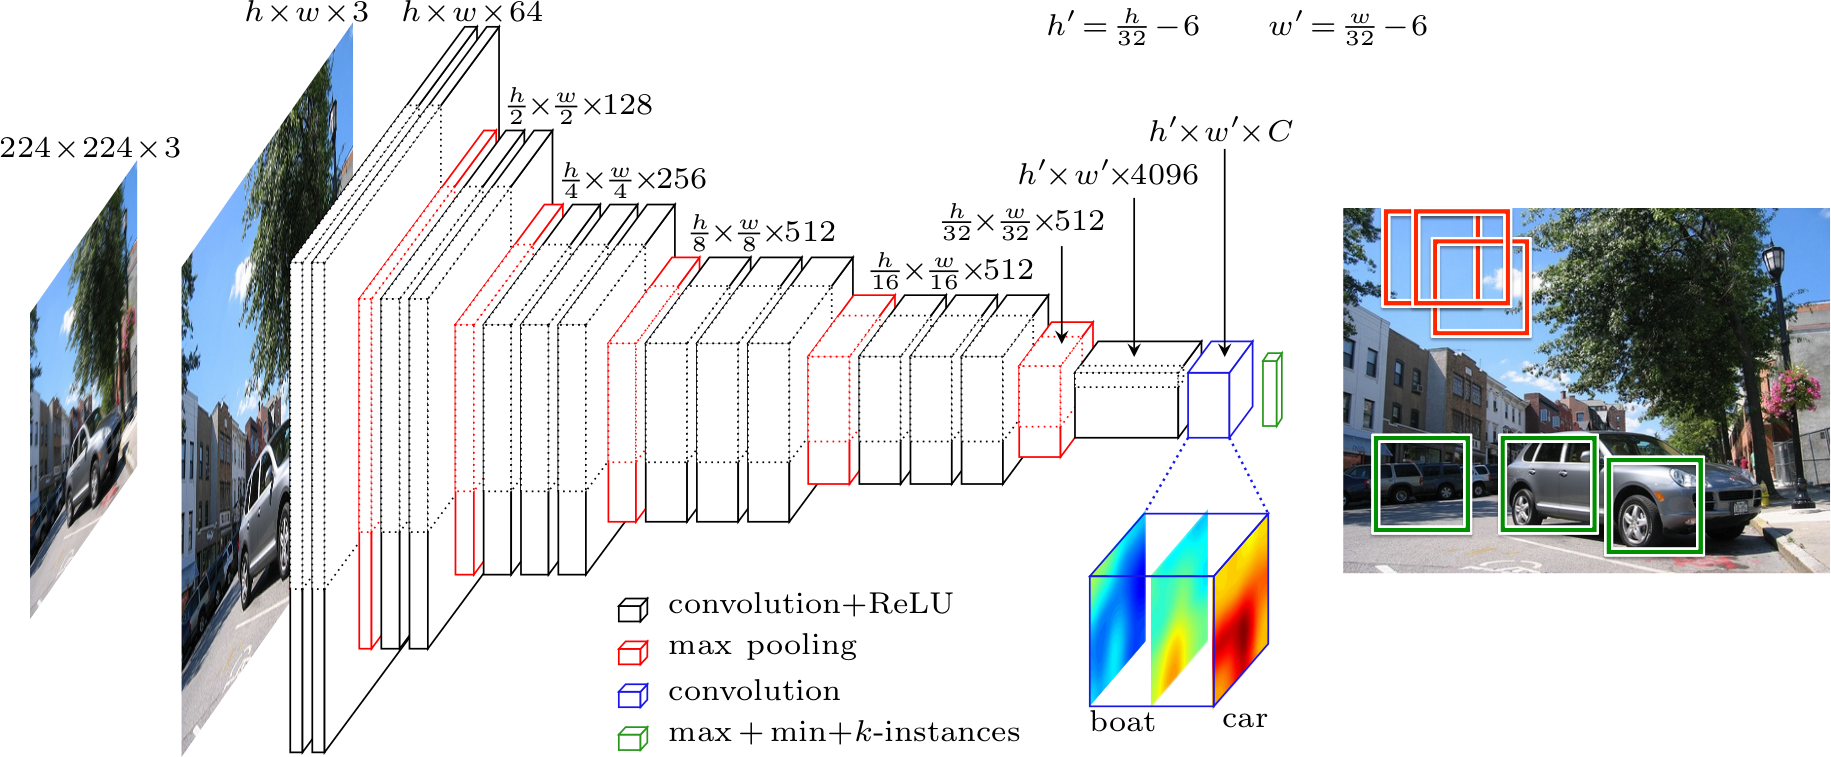
\includegraphics[width=1.05\linewidth]{images/archi_weldon2.png}
		\caption{\cite{durand2016weldon}}
		\label{fig:Weldon_figure1}
	\end{figure}
	\vspace{-0.4cm}
	\begin{itemize}
		\item Bag of visual regions
		\item End-to-End training
	\end{itemize}
\end{frame}

%--

\begin{frame}{Results : MIT67 (Small \& Strong Spatial Variance)}
	
	\begin{figure}[h]
		\centering
		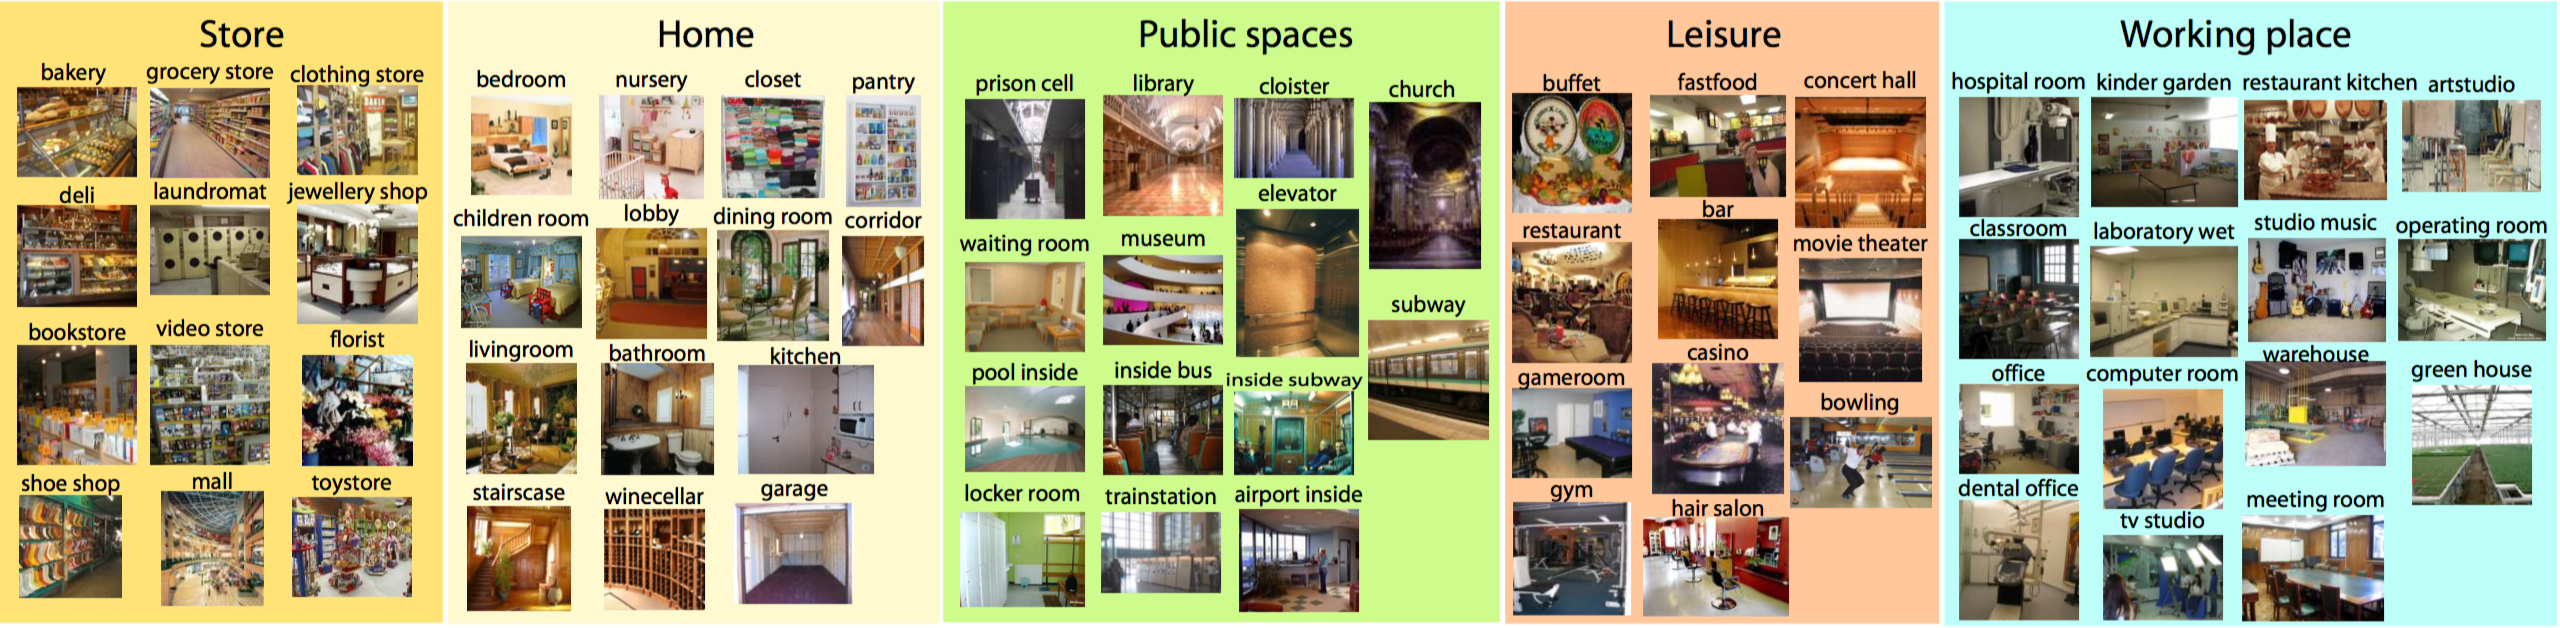
\includegraphics[width=1.05\linewidth]{images/MIT67.png}
		\caption{5360 train images, 1340 test images, 67 classes}
		\label{fig:mit67}
	\end{figure}

	\vspace{-0.5cm}
	
	\begin{table}[H]
		\small
		\centering
		\begin{tabular}{|c|c|c|}
			\hline
			Model & Method & Test Top1 (\%) \\ \hline \hline
			%--249 280 320 374 448 560 747
			Vgg16 & Extraction & 70.30 \\
			Vgg16 & Fine Tuning & 70.60 \\ \hline
			Vgg16 & WELDON & 74.10 \\
			\textbf{Vgg16} & \textbf{Ensemble \& WELDON} & \textbf{78.00} \\
			\hline
		\end{tabular}
				%\caption{Good Accuracy}
		\label{table:weldon1}
	\end{table}
	
\end{frame}



\section{Conclusion} \subsection{}\label{}

\begin{frame}{Conclusion}
	
	\begin{block}{CNNs on medium and small datasets}
	\begin{itemize}
		\item \textbf{Fine Tuning \& Ensemble > All}
		\item \textbf{Strong spatial variance $\rightarrow$ WELDON \& Ensemble}
		\item Intuition is not enough, we need theoretical proofs: \\
			\hspace{0.5cm} - How CNNs converge with non convex loss ?\\
			\hspace{0.5cm} - How 140M params CNNs avoid overfitting ?

	\end{itemize}
	\end{block}
	\vspace{-0.3cm}
	\begin{block}{\small Contributions are welcome ! (\url{github.com/Cadene/torchnet-vision})}
	\begin{itemize}
		\item Pretrain models, usual datasets, online data augmentation
		\item \href{https://github.com/Cadene/torchnet-vision/blob/master/example/mit67finetuning.lua}{\underline{Fine tuning implementation}}
		\item \href{https://github.com/Cadene/torchnet-deep6/blob/master/src/main/mit67/weldon.lua}{\underline{Weldon implementation}}

		
	\end{itemize}
	\end{block} 
\end{frame}


\section{References} \subsection{}\label{references}

\begin{frame}[allowframebreaks]{References}
	
	\printbibliography[heading=none]
	
\end{frame}


